\begingroup
\renewcommand\thechapter{B}
\titleformat{\chapter}[display]
{\normalfont\huge\bfseries}{}{20pt}{\Huge}
\setcounter{section}{0}
\setcounter{figure}{0} 

\chapter*{Appendix B - MongoDB and VS Code}
\addcontentsline{toc}{chapter}{Appendix B - MongoDB and Visual Studio Code}

Throughout the course of this project's development, Visual Studio Code ("VSCode") was used as the IDE.
VSCode allows its features to be expanded through extensions on its community marketplace. To assist greatly with 
this project's development, the MongoDB VSCode extension was installed, which provides the interface shown in 
Figure \ref{fig:VSCodeMongoUI}

\begin{figure}[H]
    \centering
    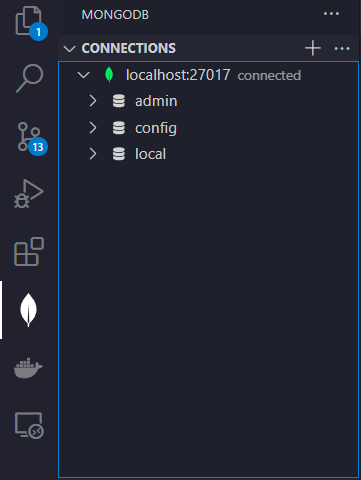
\includegraphics[width=0.5\textwidth]{VSCode/MongoExtensionUI}
    \caption{The MongoDB extension interface within VSCode.\label{fig:VSCodeMongoUI}}
\end{figure}


% This maybe doesn't actually have to be an appendix, though I wasn't sure where would be best to address this topic.
% Consider that it also doesn't really need addressing at all unless you use a hyper-specific feature.

\endgroup
